
Let \( y = \frac{1}{x} \) for \( x \geq 1 \). The function is continuous, strictly decreasing, and asymptotic to zero. As \( x \to \infty \), its value becomes arbitrarily small but remains strictly positive. Rotating this curve around the \( x \)-axis produces a surface of revolution. Each point \( (x, y) \) sweeps out a circle of radius \( y \), generating a solid that narrows indefinitely as it extends without bound in the horizontal direction. This shape is known as Torricelli’s trumpet.

\begin{figure}[h!]
\centering
\begin{tikzpicture}[scale=1.1, domain=1:6, samples=100]
  \draw[->] (0,0) -- (6.5,0) node[right] {$x$};
  \draw[->] (0,0) -- (0,1.5) node[above] {$y$};
  \draw[thick, blue] plot (\x,{1/\x}) node[right] {$y=\frac{1}{x}$};
  \draw[dashed] (1,0) -- (1,1);
  \node at (1,-0.2) {$1$};
\end{tikzpicture}
\caption{The generating curve \( y = \frac{1}{x} \) for \( x \ge 1 \).}
\end{figure}

The volume enclosed by this object is computed by integrating the cross-sectional areas of its infinitesimal disks. At horizontal position \( x \), the area of the disk is \( \pi y^2 = \pi/x^2 \). The volume element is \( \pi/x^2 \, dx \), and the total volume is
\[
\int_1^\infty \pi \cdot \frac{1}{x^2} dx = \pi.
\]
The integral converges due to the decay rate of the integrand: for \( p > 1 \), the improper integral \( \int_1^\infty \frac{1}{x^p} dx \) is finite. The trumpet can be filled with a finite quantity of material.

To compute surface area, one must measure the arc length of the generating curve and sum the areas of the resulting surface ribbons under rotation. The infinitesimal arc length is
\[
ds = \sqrt{1 + \left( \frac{dy}{dx} \right)^2} dx = \sqrt{1 + \frac{1}{x^4}} dx,
\]
and the circumference at position \( x \) is \( 2\pi y = 2\pi/x \). The surface area element is
\[
dA = 2\pi \cdot \frac{1}{x} \cdot \sqrt{1 + \frac{1}{x^4}} dx.
\]
The total surface area satisfies
\[
\int_1^\infty 2\pi \cdot \frac{1}{x} \cdot \sqrt{1 + \frac{1}{x^4}} dx > \int_1^\infty \frac{1}{x} dx = \infty.
\]
The trumpet has infinite surface area. The boundary accumulates too slowly to suppress divergence.
\begin{figure}[h!]
\centering
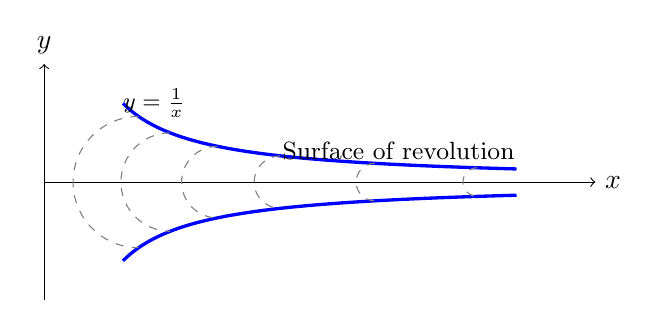
\begin{tikzpicture}[scale=1.0]
  % Axes
  \draw[->] (0,0) -- (7,0) node[right] {$x$};
  \draw[->] (0,-1.5) -- (0,1.5) node[above] {$y$};

  % Generating curve
  \draw[very thick, blue, domain=1:6, samples=100] plot (\x,{1/\x});

  % Mirror curve
  \draw[very thick, blue, domain=1:6, samples=100] plot (\x,{-1/\x});

  % Rotational bands (just visual cues)
  \foreach \x in {1.2, 1.6, 2.2, 3, 4.2, 5.5} {
    \draw[dashed, gray] (\x,{1/\x}) arc[start angle=90, end angle=270, radius={1/\x}];
  }

  \node at (1.4,1) {\footnotesize $y = \frac{1}{x}$};
  \node at (4.5,0.4) {\small Surface of revolution};
\end{tikzpicture}
\caption{The surface of revolution obtained by rotating \( y = \frac{1}{x} \) around the \( x \)-axis.}
\end{figure}


This difference in behavior is governed by the decay rates of the integrands. Volume accumulation involves \( 1/x^2 \), which lies above the convergence threshold. Surface area involves \( 1/x \), which lies exactly at the divergence boundary. The geometry is smooth throughout; the asymmetry arises analytically from how surface and volume integrate at large distances.

The trumpet is often used to introduce the so-called painter’s paradox (or Gabriel's horn): the solid can be filled with a finite amount of paint, but its surface cannot be painted using any finite amount. This formulation confuses physical and mathematical models. Mathematical paint has no thickness and can be distributed over arbitrary areas. Physical paint consists of discrete particles and cannot form zero-thickness coatings. The divergence of surface area is a property of the continuous model and implies no contradiction. It reveals how bounded integrals depend not on spatial extent but on integrand behavior.

Richard Kaufmann has offered a complementary framing based on dimensional construction. Any finite volume consists of an uncountable accumulation of two-dimensional area layers. One may imagine a cube as an infinite stack of zero-thickness sheets, each with area. When the cube melts into a film, these areas reassemble into an unbounded surface. From this perspective, infinite surface content is structurally embedded in every three-dimensional region, even when the total volume is finite. The trumpet’s behavior follows from this general principle. Its finite volume does not preclude its surface from being assembled from an unbounded number of infinitesimal circumferences.

The same structure appears in other geometric examples. The region under \( y = \frac{1}{x^2} \) for \( x \geq 1 \) encloses finite area but has infinite arc length. The integrand \( \sqrt{1 + \left( \frac{d}{dx} \frac{1}{x^2} \right)^2} \) behaves asymptotically like 1, and the integral diverges. Infinite boundary extent is consistent with finite content when the accumulation is sufficiently slow.

In physical systems, similar structures govern accumulation. A wavefunction may decay slowly enough to cover all space yet be square-integrable. A gravitational or electric field may extend to infinity while having finite energy. In fractal geometry, iterative boundary growth yields finite area with unbounded perimeter. These effects depend on decay rate and dimensional weighting, not on the apparent size of the object.

Higher-dimensional versions of the trumpet preserve this pattern. In four-dimensional space, a hypersolid generated by rotating a surface about a hyperplane may have finite four-volume but infinite three-dimensional boundary measure. For convergence in \( n \)-volume, the integrand must decay faster than \( 1/x^n \); for boundary measure, faster than \( 1/x^{n-1} \). The trumpet corresponds to the case \( n = 3 \). Its volume accumulates over \( 1/x^2 \), its surface over \( 1/x \). One integral converges, the other diverges.

The divergence of surface area is not a limitation or anomaly. It is a consequence of how geometric measures scale under integration. Infinite structure appears naturally from consistent accumulation over unbounded domains. The trumpet is an instance of this general behavior.

\clearpage
garbage
\clearpage
garbage
\clearpage